
\section{Formula Complexity}
\label{sec:formula}

Formula complexity is a ``low-powered'' version of Kolmogorov complexity\footnote{The standard text for Kolmogorov complexity is Li and Vitanyi\cite{Li}}.  Kolmogorov complexity
allows the full power of a programming language to be put to bear in describing
how an output is produced.  In particular, Kolmogorov complexity allows for the definition and
application of functions as well as conditional statements.  In our language,
the only things which can be used are formulae with a boolean result
involving only the logical atoms {\tt and}, {\tt or}, {\tt not}, {\tt true},
and {\tt false}, as well as the numerical atoms of {\tt 0}, {\tt 1}, {\tt x},
{\tt y}, {\tt +}, {\tt *}, and {\tt <}.

Because formula complexity disallows loops and function definitions, every
formula represents a terminating program.  Even more, since the domain of all
of the operators is total, this means that every well-typed formula represents
a non-crashing program\footnote{This is why the division and modulus operators
were excluded, as {\tt 12 mod 0} and {\tt 12 / 0} result in a crashing program
rather than a value.}.  Thus, in exchange for ``powering down'' Kolmogorov complexity, we can
actually enumerate and test all formulae, without worrying about infinite loops
or crashes.

Each formula evaluates to a boolean and involves the variables $x$ and/or $y$.
Therefore, to create a $3\times3$ artwork from a formula, simply evaluate the formula
at all of the points $(x,y) = (0,0)$, $(x,y) = (0,1)$, $(x,y) = (0,2)$, $(x,y)
= (1,0)$, $\ldots$, and $(x,y) = (2,2)$.  Where the formula evaluates to true,
set the corresponding square on the art to black, and where the formula is
zero, set the square to white.  Every artwork has multiple formula which
produce it.  The formula complexity of an individual artwork is the smallest
such formula.

As an example, the all-black is produced by the formula {\tt true}, {\tt not
false}, {\tt true or false}, and many many others.  However, because the
smallest such formula consists of just one atom, the formula complexity of the
all-black artwork is 1.  From this example (and from the definition), we see
that formula complexity is a property of an artwork, not a formula.  The
formula complexity is defined as the size of the smallest formula able to
produce the output in question. 

\subsection{Generating The Art}

To generate all the art, we first generate all well-typed boolean formulae, in
order of size.  Then, for each formula, we generate its corresponding artwork.
If this is the first time that artwork has been generated, we then know that
the formula complexity of the artwork is equal to the size of the formula just
used.  Generating all the \twoxtwo\ formulae revealed some hidden structure to our
results.

\subsubsection{All the \twoxtwo\ Art}

From Figure~\ref{fig:2x2}, some things are immediately obvious.  First of all,
as might match one's intuition, the all-black and all-white pictures are the
least complex pictures.  Secondly, one can see that if a formula of size $n$
exists to create a certain picture, then that picture's inverse has a
complexity of one of $n-1$, $n$, or $n+1$.  Examples of this last phenomenon
can be seen between levels 7 and 8, as well as between levels 3 and 4.  This occurs
for the simple reason that adding one symbol ({\tt not}) creates a picture's
inverse.  Also, somewhat intriguingly, we can see gaps at 2 and 6.  Although
there are formulae of size 2, none of those formulae produce a picture that has
not been already produced by formulae of a smaller size e.g {\tt (not true)}
and {\tt (not false)} are more succinctly expressed as {\tt false} and {\tt
true}.

Also visible in our results is that if an artwork has formula complexity of
$n$, then the diagonal flip of that artwork also has formula complexity of $n$,
because exchanging $x$ and $y$ results in a formula of exactly the same size.
This can be seen in levels 3, 4, and 5 of Figure~\ref{fig:2x2}.

\begin{figure}
\begin{center}
\begin{tabular}{r c l}
Formulae & Level & Pictures \\
\tiny{none} & 0 & empty \\
\tiny{(true), (false)} & 1 &
    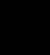
\includegraphics[width=.25in]{../presentation/2x2/Shape1LVL1.png}~
    
\includegraphics[width=.25in]{../presentation/2x2/Shape2LVL1.png} \\
\tiny{none} & 2 & empty \\
\tiny{($<$ x 1), ($<$ y 1), ($<$ x y), ($<$ 0 x), ($<$ 0 y), ($<$ y x)} & 3 & 
    
\includegraphics[width=.25in]{../presentation/2x2/Shape1LVL3.png}~
    
\includegraphics[width=.25in]{../presentation/2x2/Shape2LVL3.png}~
    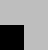
\includegraphics[width=.25in]{../presentation/2x2/Shape5LVL3.png}~
    
\includegraphics[width=.25in]{../presentation/2x2/Shape6LVL3.png}~
    
\includegraphics[width=.25in]{../presentation/2x2/Shape3LVL3.png}~
    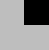
\includegraphics[width=.25in]{../presentation/2x2/Shape4LVL3.png}\\
\tiny{(not ($<$ x y)), (not ($<$ y x))} & 4 & 
    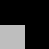
\includegraphics[width=.25in]{../presentation/2x2/Shape2LVL4.png}~
    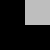
\includegraphics[width=.25in]{../presentation/2x2/Shape1LVL4.png} \\
\tiny{($<$ (y + x) 1), ($<$ (y * x) 1), ($<$ 0 (y + x)), ($<$ 1 (y + x))} & 5 & 
    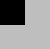
\includegraphics[width=.25in]{../presentation/2x2/Shape2LVL5.png}~
    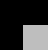
\includegraphics[width=.25in]{../presentation/2x2/Shape1LVL5.png}~
    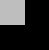
\includegraphics[width=.25in]{../presentation/2x2/Shape3LVL5.png}~
    
\includegraphics[width=.25in]{../presentation/2x2/Shape4LVL5.png} \\
\tiny{none} & 6 & empty \\
\tiny{(or ($<$ y  x) ($<$ x  y))} & 7 &
    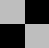
\includegraphics[width=.25in]{../presentation/2x2/Shape1LVL7.png}\\
\tiny{(not (or ($<$ y  x) ($<$ x  y)))} & 8 &
    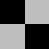
\includegraphics[width=.25in]{../presentation/2x2/Shape1LVL8.png}
\end{tabular}
\end{center}

\caption{All the \twoxtwo\ art with its corresponding complexity.}
\label{fig:2x2}
\end{figure}

After generating all \twoxtwo\ artworks, we found that the artworks were too
small for people to feel comfortable discussing those artworks' visual
complexity.  Therefore, we set our sights higher.

\subsubsection{All the \threexthree\ Art}

Generating all of the \threexthree\ art proved to be a more significant
computational challenge.  Even with some rudimentary pruning, we still had tens
of billions of formulae to check.  Our preliminary results may be seen in
Figure~\ref{fig:3x3}.  Note that although there were no new artworks in level 6
in the \twoxtwo\ results, there are new artworks at that level in the
\threexthree\ artworks --- these new artworks differ from smaller ones only in
their last column or row, and so these differences were not relevant to the
\twoxtwo\ case.

\begin{figure}
\begin{center}
\begin{sideways}
\input{3x3table.tex}
\end{sideways}
\end{center}

\caption{All the \threexthree\ art with its corresponding complexity.}
\label{fig:3x3}
\end{figure}

After generating all the \threexthree\ artworks, we wished to discover whether
our notion of formula complexity had anything to do with visual complexity.

